\documentclass{scaffold/sigchi}
\usepackage{pifont} % Check marks
\newcommand{\cmark}{\ding{51}} % So we can use \cmark instead of \ding{51}
\newcommand{\xmark}{\ding{55}}

% Title
\def\plaintitle{Investigating How Different Rewards Controlled by a Chatbot Effect the Formation of New Habits}

% Authors as plain text
\def\plainauthor{First Author, Second Author, Third Author,
  Fourth Author, Fifth Author, Sixth Author}
\def\emptyauthor{}
\def\plainkeywords{habit formation; behaviour change; chatbot; rewards; modalities; visual; audio; visual-audio.}
\def\plaingeneralterms{Documentation, Standardization}
  \usepackage{pgfplots}
  \pgfplotsset{compat=1.12}

% Use this section to set the ACM copyright statement (e.g. for
% preprints).  Consult the conference website for the camera-ready
% copyright statement.

% Copyright
\CopyrightYear{2017}
%\setcopyright{acmcopyright}
\setcopyright{acmlicensed}
%\setcopyright{rightsretained}
%\setcopyright{usgov}
%\setcopyright{usgovmixed}
%\setcopyright{cagov}
%\setcopyright{cagovmixed}
% DOI
\doi{http://dx.doi.org/10.475/123_4}
% ISBN
\isbn{123-4567-24-567/08/06}
%Conference
\conferenceinfo{CHI'18,}{April 21--26, 2018, Montreal, Canada}
%Price
% \acmPrice{\$15.00}

% Use this command to override the default ACM copyright statement
% (e.g. for preprints).  Consult the conference website for the
% camera-ready copyright statement.

%% HOW TO OVERRIDE THE DEFAULT COPYRIGHT STRIP --
%% Please note you need to make sure the copy for your specific
%% license is used here!
% \toappear{
% Permission to make digital or hard copies of all or part of this work
% for personal or classroom use is granted without fee provided that
% copies are not made or distributed for profit or commercial advantage
% and that copies bear this notice and the full citation on the first
% page. Copyrights for components of this work owned by others than ACM
% must be honored. Abstracting with credit is permitted. To copy
% otherwise, or republish, to post on servers or to redistribute to
% lists, requires prior specific permission and/or a fee. Request
% permissions from \href{mailto:Permissions@acm.org}{Permissions@acm.org}. \\
% \emph{CHI '16},  May 07--12, 2016, San Jose, CA, USA \\
% ACM xxx-x-xxxx-xxxx-x/xx/xx\ldots \$15.00 \\
% DOI: \url{http://dx.doi.org/xx.xxxx/xxxxxxx.xxxxxxx}
% }

% Arabic page numbers for submission.  Remove this line to eliminate
% page numbers for the camera ready copy
% \pagenumbering{arabic}

% Load basic packages
\usepackage{balance}       % to better equalize the last page
\usepackage{graphics}      % for EPS, load graphicx instead 
\usepackage[T1]{fontenc}   % for umlauts and other diaeresis
\usepackage{txfonts}
\usepackage{mathptmx}
\usepackage[pdflang={en-US},pdftex]{hyperref}
\usepackage{color}
\usepackage{booktabs}
\usepackage{textcomp}

% Some optional stuff you might like/need.
\usepackage{microtype}        % Improved Tracking and Kerning
% \usepackage[all]{hypcap}    % Fixes bug in hyperref caption linking
\usepackage{ccicons}          % Cite your images correctly!
% \usepackage[utf8]{inputenc} % for a UTF8 editor only

% If you want to use todo notes, marginpars etc. during creation of
% your draft document, you have to enable the "chi_draft" option for
% the document class. To do this, change the very first line to:
% "\documentclass[chi_draft]{sigchi}". You can then place todo notes
% by using the "\todo{...}"  command. Make sure to disable the draft
% option again before submitting your final document.
\usepackage{todonotes}






% llt: Define a global style for URLs, rather that the default one
\makeatletter
\def\url@leostyle{%
  \@ifundefined{selectfont}{
    \def\UrlFont{\sf}
  }{
    \def\UrlFont{\small\bf\ttfamily}
  }}
\makeatother
\urlstyle{leo}




% To make various LaTeX processors do the right thing with page size.
\def\pprw{8.5in}
\def\pprh{11in}
\special{papersize=\pprw,\pprh}
\setlength{\paperwidth}{\pprw}
\setlength{\paperheight}{\pprh}
\setlength{\pdfpagewidth}{\pprw}
\setlength{\pdfpageheight}{\pprh}

% Make sure hyperref comes last of your loaded packages, to give it a
% fighting chance of not being over-written, since its job is to
% redefine many LaTeX commands.
\definecolor{linkColor}{RGB}{6,125,233}
\hypersetup{%
  pdftitle={\plaintitle},
% Use \plainauthor for final version.
%  pdfauthor={\plainauthor},
  pdfauthor={\emptyauthor},
  pdfkeywords={\plainkeywords},
  pdfdisplaydoctitle=true, % For Accessibility
  bookmarksnumbered,
  pdfstartview={FitH},
  colorlinks,
  citecolor=black,
  filecolor=black,
  linkcolor=black,
  urlcolor=linkColor,
  breaklinks=true,
  hypertexnames=false
}

% create a shortcut to typeset table headings
% \newcommand\tabhead[1]{\small\textbf{#1}}

\title{\plaintitle}




% Authors on paper
\numberofauthors{3}
\author{%
  \alignauthor{Leave Authors Anonymous\\
    \affaddr{for Submission}\\
    \affaddr{City, Country}\\
    \email{e-mail address}}\\
  \alignauthor{Leave Authors Anonymous\\
    \affaddr{for Submission}\\
    \affaddr{City, Country}\\
    \email{e-mail address}}\\
  \alignauthor{Leave Authors Anonymous\\
    \affaddr{for Submission}\\
    \affaddr{City, Country}\\
    \email{e-mail address}}\\
}

\begin{document}

\maketitle

\begin{abstract}
Habit formation systems usually reward users, after they complete a habit. This paper compares three types of positive reinforcement rewards from two modalities to see how they effect habit formation. A prototype was constructed to help users track habits, gather data about users activity and send rewards from two different modalities: visual and auditory. The aim is to explore how the reward from each modality effects habit formation. 36 users evaluated the bot during a 3-week period, followed by 1-week without interaction. Four user groups received different types of rewards from a different mode: no reward, visual, auditory, and visual-auditory combined. The evaluation trial tested how each type of reward effected users habit automaticity by using a validated questionnaire and analysing users data that was collected by the bot. The trial revealed the effectiveness of these chosen rewards on users habit strength and analysis on the motivation about each modality. Semi-structured user interviews, combined with the data analysis, found at the end of the 4-week period: i) visual rewards had the highest increase in habit strength, ii) ..., finally, iii) participants found interacting with the chatbot fun.
\end{abstract}

\category{H.5.2}{Information interfaces and presentation (e.g. HCI)}{User Interfaces, auditory (non-speech) feedback, interaction styles}
\category{J.4}{Social and Behavioural Sciences}{Psychology}

\keywords{\plainkeywords}


\section{Introduction}        
Habits are automatic actions that require little effort. A simple action such as turning on the light to a room happens automatically, even if the light is already on.
Forming a new automatic action is difficult, and requires three elements: contextual cues, positive reinforcement and repetition~\cite{article_experiences_of_habit_formation}. Contextual cues are existing routines that trigger the person to perform the action. Positive reinforcement rewards the person encouraging them to perform the action again, until it forms into a habit. Finally, repetition is needed --- as habits, on average, take up to 66 days to form~\cite{article_how_habits_formed_modelling_habit_formation}.
However, people still fail at forming new positive habits and give up, often due to their lack of routine~\cite{article_promoting_habit_formation, article_the_habitual_consumer}.

Mobile technology can help people stick to a routine. By associating the desired action with contextual information to develop a cue. It can positively reinforce with rewards after completing the action. Finally, it can send repetitive checks, that adjust to changes in environment.
Yet most existing mobile habit formation systems are not always built on theory~\cite{article_beyond_self_tracking_designing_apps, article_dont_kick_habit}, and usually build repetitive actions rather than habit automaticity.
Therefore, people become dependent on technology, and when the system is eventually removed, habit performance decreases. Building habit automaticity is the key that removes this dependency~\cite{article_beyond_self_tracking_designing_apps}.\newline
\newline
Automaticity can be increased by building motivation to complete the action~\cite{article_a_self_efficacy, article_meta_analytic_review_intrinsic_motivation}.
Motivation can be encouraged by rewarding users with positive reinforcement to grant them satisfaction after completing the action.
However, these are not enough to be successful, the reward and delivery type are crucial to success.\newline
\newline
Monetary rewards (extrinsic rewards) hinders motivation~\cite{article_meta_analytic_review_intrinsic_motivation}, whereas, satisfaction-based rewards (intrinsic rewards) benefits the person and should be preferred~\cite{article_meta_analytic_review_intrinsic_motivation}.
The type of delivery should suit each individual user requiring a choice of delivery to be available.
Different research~\cite{article_user_centred_multimodal_reminders} shows how interaction with users should span different modalities to suit the needs to users.
This paper combines knowledge from these two domains to focus on how intrinsic positive reinforcement rewards from different modalities affect people's habit strength.

To evaluate our hypothesis we present a tool to help test it: a mobile technology chatbot to deliver rewards from different modalities.
These rewards are delivered using the bot to present a novel behaviour change method for interacting with users.
Chatbots are a method of communicating with a computer system using natural language, providing deeper integration into users mobile phone and be deployed into into messaging services users are familiar with, such as Facebook Messenger.
The chatbot design is based on a combined set of theory-based design requirements;
one for building habit formation apps that aim to increase habit automaticity and one for increasing motivation with intrinsic rewards.\newline
\newline
An evaluation trial tests the prototype during a 4-week controlled period to measure user's habit strength.
36 participants engaged in daily activity with the bot for 3 weeks, then for a further 1-week all bot interaction was suspended to test if users continued with their chosen habit after removing the bot.
The chatbot provides habit tracking with three combinations of rewards, visual, auditory and visual-auditory combined.
Participants were split into four groups: one control group without rewards and three groups receiving different combinations.
The evaluation trial tested the success of the chatbot by measuring reward modes compared with habit strength after the trail. These were compared with the results from the control group to prove the effectiveness of each reward mode.


\section{Background}
To understand how to build a tool that supports habit formation, we must discuss how people fundamentally form habits.

\subsection{Habit Formation}
Psychology defines habits as learned automatic cue-response actions, such actions that will perform automatically in response to another action or trigger that has been actioned repeatedly in the past~\cite{article_the_habitual_consumer}. People must keep to strict strategies and perform an action repeatedly before it occurs with little concious thought~\cite{article_promoting_habit_formation}. Habit formation requires behaviour change. Three elements are needed to make this change permanent: repetition, contextual cues and positive reinforcement~\cite{article_experiences_of_habit_formation}.

\subsubsection{Repetition}
Lally~et~al.~\cite{article_how_habits_formed_modelling_habit_formation} conducted a test on how long it takes for an action to become automatic, showing that the process of creating a new habit takes on average 66 days of repetitive use. The easier the action, the shorter the before the action turns into a habit, from drinking water (18 days), to going to the gym (254 days)~\cite{article_how_habits_formed_modelling_habit_formation}. However, applying the other two elements is needed before the action develops into a habit.

\subsubsection{Contextual Cues}
An existing routine acts as a trigger to motivate the desired action. Context from that routine serves as the cue for the trigger. For example, if you wanted to adopt a stretching habit, you could attach it onto an existing habit like brushing your teeth. The contextual cue of brushing your teeth will trigger you to stretch. Attaching habits onto existing event-based cues are easier to remember~\cite{article_implementation_intentions_multicue}, when compared with time-based habits, e.g. stretch every 4 hours. These help connect the contextual information with the action and builds habit automaticity~\cite{article_implementation_intentions}. Finally, when designing behaviour change interventions multi-cue routines have shown to be more effective than a single cue~\cite{article_understanding_use_contextual_cues_design_impl}.

\subsubsection{Positive Reinforcement}
Self-efficacy (the belief in ones ability to succeed) plays a large part in forming habits~\cite{article_a_self_efficacy} and some research suggests it is the main part of behaviour change. Rewards give people this experience by feeding back their success of their action. Rewarding a person with positive reinforcement, strengthens the habit by giving the feeling of satisfaction~\cite{article_promoting_habit_formation}. However, the type of reward matters, as rewards that benefit the person with satisfaction (intrinsic rewards) should be used over monetary gains (extrinsic rewards), because extrinsic rewards have a negative effect on motivation~\cite{article_meta_analytic_review_intrinsic_motivation}, particularly in relation to interesting tasks. Therefore, this paper focuses on positive reinforcement intrinsic rewards.

\begin{figure}
  \centering
  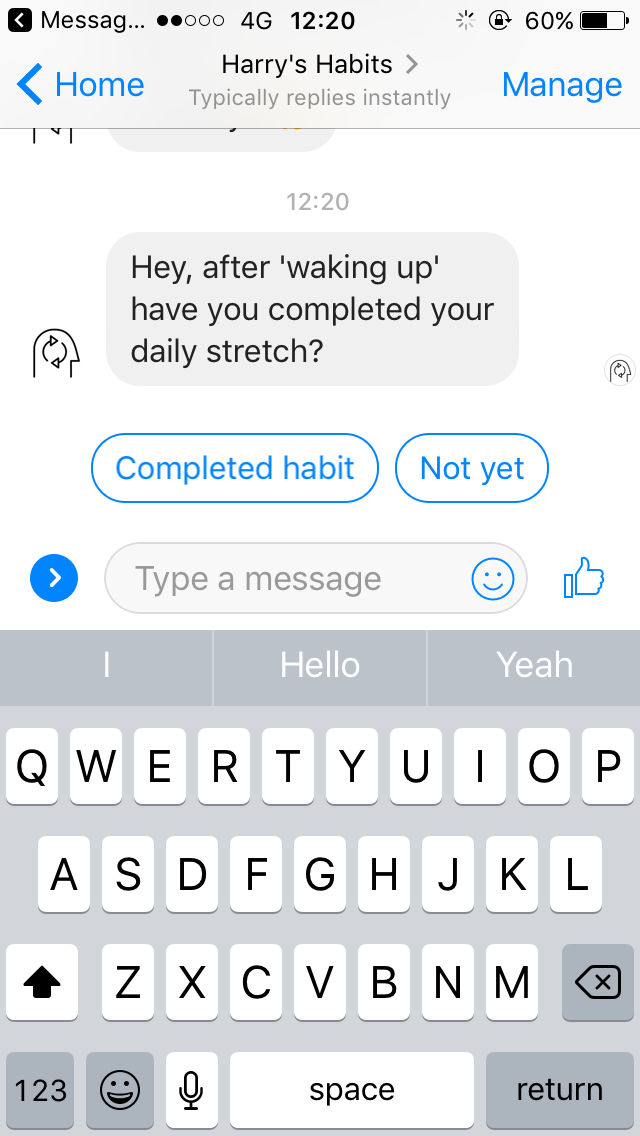
\includegraphics[width=0.47\columnwidth]{figures/reminder.png}
  \hspace{5px}
  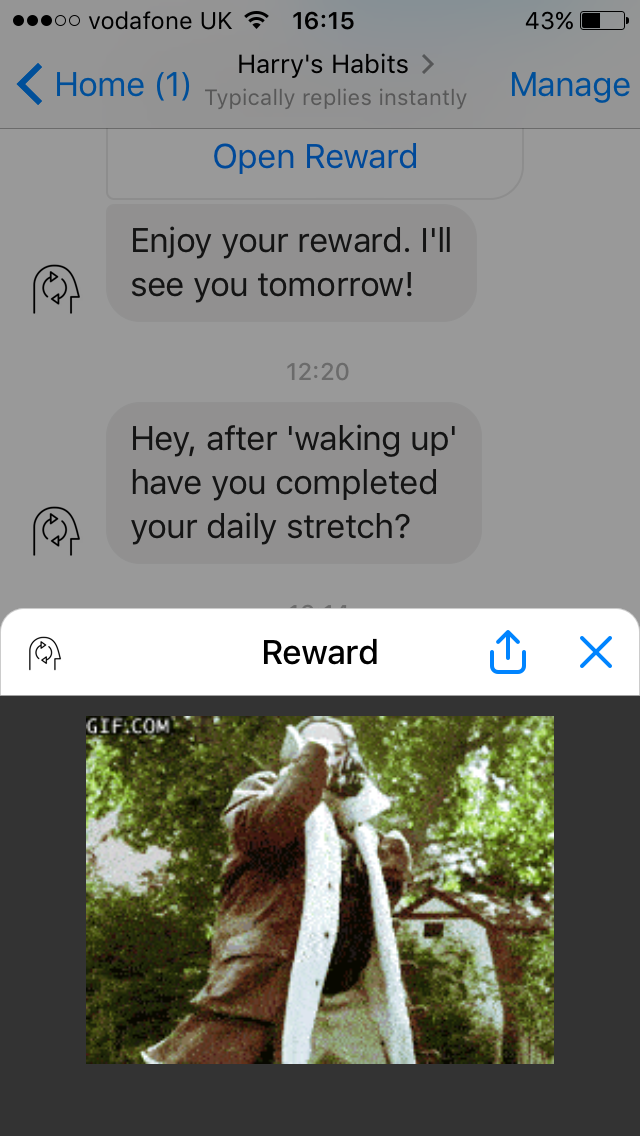
\includegraphics[width=0.47\columnwidth]{figures/reward-visual.png}
  \caption{Prototype delivering a visual reward after a user has marked their habit as completed.}~\label{fig:setup}
\end{figure}

\subsection{Rewards}
TODO: Compare different reward types. We will focus only on positive reinforcement rewards, however, there are lots of different types...

TODO: Reward rationale, stating the rise of social media, with memes, these rewards seem appropriate for a chatbot.

Previous habit formation research~\cite{article_understanding_use_contextual_cues_design_impl} shows how different \textit{contextual cues} better support behaviour change, compared with a single mode. But, we want to see if using different types of \textit{positive reinforcement} rewards better supports behaviour change, compared with single mode. We want to map habit rewards across different modalities, to present users with the same reward type from a different modality.
This allows us to test the different types of modalities and how they effect behaviour change.
The next section discusses methods of interaction in practice.

\subsection{Modalities}
The three chosen modes, visual, auditory, and visual-auditory combined, are chosen for testing. Feedback from each of these different modalities, has been shown to impact the task performance for small tasks~\cite{chi_oussama_tap_the_shapetones}. TODO join the next paragraphs into this one.


`Multi-modal systems are required for user interaction'~\cite{article_user_centred_multimodal_reminders} states research into comparing uni-modal reminders systems with multi-modal.
They suggests a need for `highly flexible and contextualised multi-modal and multi-device reminder systems'~\cite{article_user_centred_multimodal_reminders}.
Although this study focused on the elderly, so the need to multiple modalities was important because some peoples sensory modalities decline with age,
this principle still holds true for general case reminder systems. The study presents design guidelines for reminder systems.
These are mainly focused on users needing a choice of modalities for interacting with users, as users want a highly configurable system.
These aspects are implemented into our prototype and adapted for delivering rewards.\newline
\newline
Research into designing reminder systems for the home that interact with users in different modalities, states that
`Good reminder systems should use different modalities, because they provide alternative ways to interact with a user'~\cite{article_designing_multimodal_reminders_for_home}.
Using different modalities for interaction increases the likelihood that the information users are receiving will be more receptive to them,
and decreases the chance the interaction will be disruptive or annoying~\cite{article_designing_multimodal_reminders_for_home}.
Habit rewards should not be annoying, they should give users a feeling of satisfaction, therefore reducing the chance of disruption is another justification for using multiple modalities.

We want to compare each modality with a control group to see how habit formation is impacted. The next section looks at literature discussing the two modality types used and how they change peoples behaviour.
\subsubsection{Visual}
One study looked at improving habit consistency for how often patients took medication,
by using a visual display device that gave constant feedback~\cite{article_realtime_feedback_improving_medication_taking}.
They found that this feedback improved consistency of the habit and increasing rating of self-efficacy.
But when the device was removed, their performance dropped (from a 2-month follow up study), because users integrated the feedback display with their routines.
This habit-forming system used visual feedback to encourage consistency, however, this system shouldn't integrate visual cues into the system, otherwise users become dependent on the technology.
Users should instead build these cues outside of the system to build performance longevity after removing the system.
\subsubsection{Auditory}
Another key paper, discussed their need for different modalities when designing for the elderly~\cite{article_movipill_improving_medication_elders},
combing different sounds with high visual contrast to suit their needs, given deteriorating senses due to age.
The study showed that using different modalities for interaction gives a means of communication to people with varying levels of sense ability.
But studies have also shown people need a choice of mode when designing for interaction~\cite{article_user_centred_multimodal_reminders},
and thus the design requirements produced from this study can be applied to general applications that use multiple modalities, such as this project.
The design guidelines discuss the need for interaction consistency, such as using similar audio interaction.
Therefore visual and auditory rewards are mapped identifying a pattern across the modalities.
\subsubsection{Visual-Auditory}
Combining audio with visual can be advantageous as feedback after the completion of a simple task, as proven by lots of research, e.g.~\cite{benefits_of_audio_visual_1, benefits_of_audio_visual_2}. A meta-analysis of 43 multi-modal studies~\cite{comparing_modalities_effects_of_visual_auditory} revealed that it was the most effective to increase performance, when a single task is being performed, when compared with visual or auditory feedback alone. However, care needs to be taken when adding an extra modality as this research states that 'visual feedback improved task performance, but not error rate'~\cite{comparing_modalities_effects_of_visual_auditory}. In addition, while all modalities contribute to perceptual experience, one sense can override another if the sensory channel mediates less ambiguous information than the other~\cite{one_mode_override_another}. Finally, this combination of visual and auditory sensory channels has been shown to increase performance with complex tasks~\cite{chi_oussama_tap_the_shapetones}, therefore it will be useful to compare the success of the task with the other modes.
\subsection{Mapping Modalities}
First, the actual rewards are aimed to motivate participants to complete further habits. Gifs and audio are found from the site, with the search 'Motivation'. Each frame of the gif image is altered to match the audio frequency level. The frame is slowed down if the audio level is lower, or speed up, if the audio frequency level is higher. The relationship between the audio and the visual is inferred, therefore this mapping is \textit{semi-congruent}. The next section discusses how the tool was created and delivery methods for these rewards.
\section{Technology}
TODO briefly review these papers\cite{chi_mechanics_of_persuasive_system_design, chi_time_aware_leveraging_framing_effects, personal_tracking_of_screen_time, chi_crowd_designed_motivation}

Research ~\cite{survey_on_apps_2,survey_on_current_apps_of_steel} into how mobile systems can support habit formation and behaviour change, shows a large number of habit forming systems are mobile apps. Studies into the effectiveness of these apps has been recently conducted~\cite{article_beyond_self_tracking_designing_apps, article_dont_kick_habit} revealing that although most of these apps are rated highly, they do not ground themselves in behaviour change theory. Research into some of these apps show that habits are not sustained when the app is removed, due to the lack of habit automaticity~\cite{article_beyond_self_tracking_designing_apps}.

Two pieces of literature discuss different concrete strategies for building habit forming mobile systems that do ground themselves in theory~\cite{thesis_kathy, article_taxonomy_motivational_affordances_meaningful}. Stawarz~\cite{thesis_kathy} presented formal requirements for building habit forming apps, based on the above three elements of habit formation with the aim to build habit automaticity. Weiser et al.~\cite{article_taxonomy_motivational_affordances_meaningful} shows that `motivation is a key requirement for behaviour change' presenting five design principle requirements and six requirements about the implementation mechanics of habit forming systems that focus on rewards and motivational needs. This paper builds upon these two sets of proven design requirements, combing them into a new set of design requirements (Table~\ref{tab:requirements_mine}) for habit formation systems that focus on rewards.

\begin{table}
  \centering
  \begin{tabular}{l | l}
    {\small\textit{\#}}
    & {\small \textit{Requirement}}\\
    \midrule
    1 & Help users define a memorable strategy. \\
    2 & Give users small difficult tasks. \\
    3 & Enable competition \& comparison \& cooperation. \\
    4 & Show insights for improvements and support changes. \\
    5 & Remind them about cues and remembering strategies. \\
    6 & Reward users. \\
    7 & Disable cue reminders when behaviour is routine. \\
    8 & Check if the action has already happened. \\
  \end{tabular}
  \caption{Requirements for building mobile systems that focus on rewards.}~\label{tab:requirements_mine}
\end{table}

\subsection{Requirements}
\subsubsection{1. Help users define a memorable strategy.}
Make personalized, well defined, structured multi-cue routines \& support users choice of not setting remembering strategies. In addition, provide examples of some strategies to users.

\subsubsection*{2. Give users small difficult tasks.}
Turn the bigger habit into smaller assignments to make it more enjoyable, being careful to not make them forced. These should be user specified to support user autonomy, but should be specific and challenging to get better results.

\subsubsection*{3. Enable competition \& comparison \& cooperation.}
Friends, teams, groups, leader-boards and collections.

\subsubsection*{4. Show insights for improvements and support changes.}
Give users meaningful \& accumulated  instant feedback based on their system usage.

\subsubsection*{5. Remind them about cues and remembering strategies.}
Reminders can effectively support prospective memory in the short-term, increase the logging of health data~\cite{the_power_of_logging_mobile_notifications} and educate them about what they should perform in the long-term.

\subsubsection*{6. Reward users.}
Rewards are a good form of external motivation because they don't change the ability to perform a behaviour, unless the reward itself is a tool that increases ability. These rewards provide a strong motivational source, but like all extrinsic motivators, these are less effective for changing behaviour in the long run, because externally motivated behaviour lasts as long as the external motivator exists. Use achievements and badges as means to identify methods that enable internalisation of externally motivated behaviour.

\subsubsection*{7. Disable cue reminders when behaviour is routine.}
Relying on reminders in the long-term can hinder habit development, therefore ease off from reminders later.

\subsubsection*{8. Check if the action has already happened.}
People find it easy to forget whether an automatic task was completed, check to see if the action has already happened.

These requirements act as the basis for this paper. They are guidelines for building habit formation systems that focus on delivering rewards to build habit automaticity and motivation. This paper aims to build a tool to test how different types of rewards from different modalities effect users habit strength.

\subsection{Design}
Interaction with current habit formation systems is often via a mobile app. This creates a notable difference in the person when the system is removed~\cite{article_my_phone_is_part_of_my_soul}.
This is also the case with many mobile feedback systems that aid with behaviour change.
When we remove the system any improved performance is lost~\cite{article_dont_kick_habit, article_realtime_feedback_improving_medication_taking}. To build a system for mobile devices that meets our requirements we must review all available options.\newline
\newline
Table~\ref{table:prototype_table} summarises the available choices for developing a system for our requirements. A mobile app can supply notifications, but for each platform a completely separate app would need to be built and users would need to download the app before it would be available to them.\newline
A single cross-platform app could be constructed to reduce development time and complexity, but still users would need to download the app to start using it.\newline
A web app has the advantage of being available to all users with a web browser (with users being able to save the site to home screen), but without notifications on all platforms (iOS), it won't meet our requirements.\newline
Finally, a chatbot integrated into a popular messaging platform is easily available (if you have the messaging app already installed), simple (the user interface is already supplied), cross-platform and has notifications built in.

\renewcommand{\arraystretch}{1.5} % Increase line height of the following tables
\begin{table}
  \centering
  \begin{tabular}{ p{1.9cm} | p{1.2cm} p{2.1cm} p{1cm} p{1cm} }
 \textbf{} & \textbf{\small{Mobile App}} & \textbf{\small{Cross-Platform App}} & \textbf{\small{Web App}} & \textbf{\small{Chatbot}} \\ \hline
 \small{Notifications} & \cmark & \cmark & \xmark & \cmark \\ 
 \small{Development Time} & \small{Long} & \small{Medium} & \small{Short} & \small{Short} \\ 
 \small{High Availability} & \xmark & \xmark & \cmark & \cmark \\ 
 \small{Simplicity} & \xmark & \xmark & \cmark & \cmark \\
\end{tabular}
    \caption{Comparing different prototype mediums.}
    \label{table:prototype_table}
\end{table}

\subsection{Implementation}


The prototype was developed in node.js, built on the Facebook Messenger chatbot platform and hosted on Heroku (a free Platform-as-a-Service option). Facebook messenger encourages developers to create bots to interact with their users. These bots act as a real person with similar interaction flow, plus a few additional features, such as \textit{Quick Replies} for revealing a list of options to a user. `Quick Replies provide a way to present buttons to the user in response to a message.'~\cite{doc_fb_quick_replies}. However, these bots would not reply like a real person, but rather would only reply if that question was pre-trained using machine learning algorithms. This technology requires the bot to be trained on a large set of data and the majority of use cases would have to be accounted for. Therefore simple call and responses were used to interact with users. The bot also tracked various data about how people logged their habits, such as what day they tracked their habit and how many times they delayed their checking messages. Next we look at how we evaluated the chatbot during a 4-week study.

\section{Study: Comparing Different Rewards}
TODO cite ~\cite{how_to_evaluate_tech_for_behaviour_change}\newline
Below we present our evaluation process, that place the prototype in the hands of real people, as recommended by validated guidelines \cite{article_mhealth}. First, we conducted an internal pilot trial to develop the strength of the prototype. Second, we ran a 4-week evaluation trial in the wild with real people who try and form a new positive habit. Finally, follow-up interviews with participants test if they continued with their habit without the bot.\newline
\newline
The 4-week evaluation trial is split into two sections. First a 3-week trial tests the success of the chatbot by evaluating the tool and the effectiveness of each modality on participants habit strength using a validated questionnaire~\cite{article_habit_measurement}. During the fourth week, chatbot interaction is removed during a 1-week follow up trial to test if participants continue with the habit. Participants were split into four groups, all groups receiving reminders, three groups receiving rewards each from a different modality, and one group (control group) don't receive any rewards.\newline
\newline
The study aims to compare how well people form new habits based on their reward modality and how the rewards delivered by the chatbot effect participants habit formation. The bot will collect the amount of habits people complete verses their reward type. Habit completion will be verified by using the SRBAI questionnaire~\cite{article_habit_measurement}---A validated set of questions to measure habit automaticity levels. This will be used to test if people are forming a habit. Finally, participant interviews will discuss the chatbot delivered rewards for further verification.

\subsection{Method}
Participants were instructed to connect with the bot via Facebook Messenger and pick a series of options. They were asked to choose a new habit they would like to develop from a list of habits of similar difficulty, divided into two categories: physical and relaxation. Then they were asked to state an existing routine they could build their new habit around, and choose a time that routine normally occurred (Morning, Afternoon, Evening). After they had answered these questions, they would be auto assigned a modality (unknowingly to users) for rewards, and they would continue with their day.

\subsubsection{Participants}
Overall 60 participants connected with the bot (pressed 'Get Started' in Facebook Messenger) on these platforms: 25 browser, iOS 18 and Android 12. They were recruited on social networks (using this landing page \url{www.harrymt.com/harryshabits}), and were mostly University students and staff.
54 people (90\%) continued interacting with the bot and started the set-up. 39 people (65\%) completed the set-up and out of these 39 people, 3 people just ignored all messages from the bot during the trial. Leaving 36 participants (66\%) that are considered active throughout and included in the final analysis. These 36 participants are 18-63 years old, (mean: 27 years old, SD: 12), 64\% Male and 30\% female, (6\% didn't say). 

\subsubsection{Design}
Participants answered the following set up questions from the bot when they connected with it:
\begin{itemize}
	\item 'What is your gender?',
    \item 'How old are you?',
    \item 'Have you used habit tracking systems before? If did they work and what were they?',
    \item 'What habit do you want to track?',
    \item 'What existing routine would you like to use?',
    \item 'What time does that routine occur?',
    \item 'Would you like to be interviewed about your experience after the study?'.
\end{itemize}

\begin{table}
  \centering
  \begin{tabular}{l l l l}
    % \toprule
    \cmidrule(r){3-4}
    {\small\textit{Modality}}
    & {\small \textit{Reward}}\\
    \midrule
    Visual & 15s gif. \\
    Auditory & 15s audio. \\
    Visual \& Auditory & 15s gif and audio. \\
    None & No reward. \\
    % \bottomrule
  \end{tabular}
  \caption{Participants are split into these four study conditions.}~\label{tab:precise_rewards}
\end{table}

A brief description accompanied these questions, to guide the participants on how to answer. The habits participants could choose were split into two categories, physical and relaxation. They were: stretching, press ups, the plank, reading, writing or meditation.\newline
\newline
The study used four conditions: visual rewards, auditory rewards, visual-auditory rewards and no rewards (control group). Participants were randomly assigned a condition by the bot (using round-robin assignment) after they \textit{competed} the set-up. Out of these remaining people who continued with the trial, the conditions were split across 36 people (100\%) into the following modalities: 14 people (39\%) visual, 9 people (25\%) visual and auditory, 7 people (19\%) auditory and 6 people (17\%) had no rewards (control group).\newline
\newline
Participants would receive a confirmation message, followed by positive reinforcement after they marked a habit as complete, unless they were in the control group, then they would only receive a confirmation message.
\begin{itemize}
\item \textit{Visual rewards}: Participants would receive a message that when tapped, would reveal a gif aimed at motivating them.
\item \textit{Auditory rewards}: Participants would receive a message that when tapped, would play a song aimed at motivating them.
\item \textit{Visual and auditory rewards}: Participants would receive a message that when tapped, would play a song and reveal a gif, aimed at motivating them.
\item \textit{No rewards (control group)}: Participants would only receive a confirmation message.
\end{itemize}

\subsubsection{Procedure}
During the 3-week period, after participants answered a few set-up questions to the bot, participants were ask to complete their chosen habit every day after their existing routine, then wait for the bot to send them a message asking them for one of two choices. One, if they completed their habit, or two, if they haven't completed it yet.\newline
\newline
Option one (completed habit): participants would receive a message thanking them, then participants not in the control group would receive a message linking them to a reward. This reward would be from the modality auto-assigned to that participant during the set-up phase (table~\ref{tab:precise_rewards}).\newline
\newline
Option two (not yet): the bot would check on the participant an hour later. This allowed for the checks to be snoozed, to ensure the new habit fit in with participants routine. If participants constantly told the bot they hadn't completed their habit yet, the bot would ask participants if they would like to change the time their routine occurred. This allowed the participants in the beginning to refine the time they would perform their habit.


After 3 weeks of daily bot interaction, all participants who completed the set up are asked to complete a subset (4-questions) of the SRBAI~\cite{article_habit_measurement} questionnaire, to measure habit automaticity levels. Then the bot interaction was suspended for 1 week. After the full 4-week period, participants were asked to complete the full SRBAI questionnaire (12-questions). Both questionnaires presented the questions on a 7-point Likert scale with answers from 'Strongly Disagree' (5) and 'Strongly Agree' (1). Higher scores indicates higher self-reported levels of automaticity. In addition, participants were asked if they could freely discuss their experience after the 4-week period. 28 volunteered and 8 interviews were carried out.

\subsection{Results}
36 participants sent a total of 1.1k messages to the bot (mean = 65 messages per participant) and the bot sent 2.7k total messages back. 184 total habits were marked as completed, with the bot issuing 69 visual rewards, 58 visual-auditory rewards and 17 auditory rewards to those participants. The control group completed 40 habits and were sent 0 rewards.\newline
\newline
Out of the 36 participants, 4 people blocked/deleted the thread during the study, 6 people blocked/deleted thread at the end of the 3-week period, after the bot messaged all users 'See you in a week'. Their data is included in this analysis.\newline
\newline
Meditation was the most popular habit chosen (12 people 33\%), followed by Press ups (8 people 22\%), then Stretching (6 people 15\%). Reading and writing were the least, only selected by 4 and 2 people respectively.\newline
\newline
Stretching (6 people 15\%) was the most completed habit based on selection (60 times), ranking 10.0 (where 10.0 = 60/6). Meditation ranked 6.25 (6.25 = 75/12) and the least were the plank and reading with 3.75 (15/4) and 1.75 (7/4) respectively.\newline
\newline
Participants (14 people 39\%) with visual rewards had the highest total number of snoozes (72 total presses to 'Not Yet'), auditory had the smallest (14 total). The control group had 55 snoozes and visual-auditory had 45 snoozes. Most people snoozed (answered 'Not Yet') in the morning (100 times), specifically mid (66) and late (27) morning.

\subsection{Key results}

\subsubsection{Rewards}


\begin{figure}
  \centering
  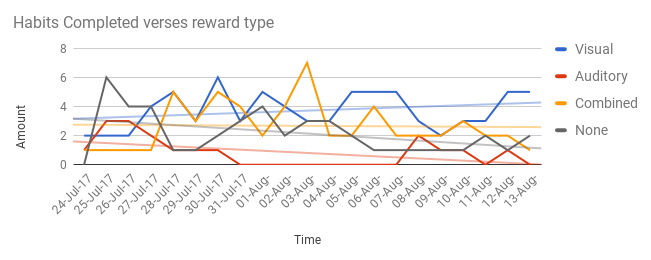
\includegraphics[width=1\columnwidth]{figures/habitscompleted-v-rewards.png}
  \caption{Habits competed per day (over 3 weeks) verses participant reward modality.}~\label{fig:habits_v_rewards}
\end{figure}

\begin{figure}
  \centering
  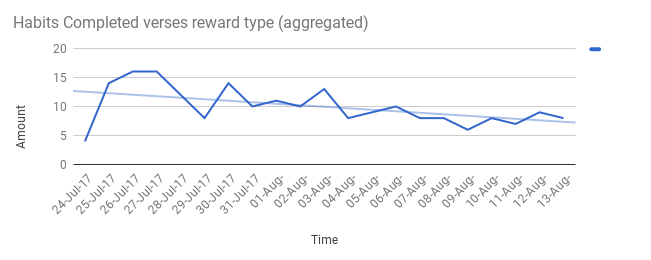
\includegraphics[width=1\columnwidth]{figures/allhabitscompleted-v-rewards.png}
  \caption{Habits completed per day (over 3 weeks) verses all participant reward types (included control group).}~\label{fig:allhabits_v_rewards}
\end{figure}


Comparing the number of people who dropped out of the study verses their reward modality, we see that 7 participants who blocked the bot had 27 visual rewards in total (mean = 3.85). 2 participants had 4 total auditory rewards (mean = 2) and 2 participants had 2 visual-auditory combined (mean = 6.5). These visual-auditory participants that dropped out had the highest amount of snoozes (24 total snoozes, 6 and 18 individually, mean = 12), compared with visual 10 total (mean = 2), and auditory with 0 snoozes.\newline
\newline
Comparing the number of habits participants completed with each reward type. We can see from graph~\ref{fig:habits_v_rewards} that participants with visual rewards completed more habits as the trial continued than any other habit.  


Under half the participants completed the modality survey (N = 12, 40\%). Likert scale was also used for various questions about participants rewards. Visual rewards had the highest score (mean = 12, SD = 3.347), visual and auditory rewards were slightly below (mean = 10.75, SD = 1.893).

\subsubsection{How many habits were completed, verses, modality type?}
Habits with visual rewards increased over time, but the rest decrease. Aggregated data shows all decreasing. However, the difference between visual rewards and habit strength show the highest increase out of all rewards.


\subsubsection{Automaticity}
Automaticity was used to measure the habit strength based on the reward used. SRBAI scores for each condition are presented in figure~\ref{fig:habit_4_item_survey1_v_survey2}.
Participants (N = 15, 41\%) completed the SRBAI (4-questions) at the end of the 3-week period. Most participants (N = 10, 27\%) completed the full 12-question SRHI 1-week later. Comparing the difference between the first questionnaire and the second: Auditory and visual rewards combined increased the most (9.4\%) from 32 SRBAI (mean = 16, SD = 2.828) to 35 SRBAI (mean = 17.5 (9.4\% increase), SD = 3.536). But, visual rewards had the highest score in both questionnaires, 73 SRBAI (mean = 14.6, SD = 4.336) for the first and 79 SRBAI (mean = 15.8, SD = 3.701) for the second (8.2\% increase). Finally, the auditory rewards had the least increase 15 SRBAI (mean = 15, SD = 0.0) to 16 SRBAI (mean = 15, SD = 0.0) (6.7\% increase) and the control group (without rewards) increased from 27 SRBAI (mean = 13.5, SD = 4.950) to 29 SRBAI (mean = 14.5, SD = 6.364) (7.4\% increase).

% 				S 1		S 2 	Increase
% NONE			27		29		7.4%
% AUDITORY		15		16		6.7%
% VISUAL		73		79		8.2%
% COMBINED		32		35		9.4%
% N: SD			4.950	6.364
% A: SD			0		0
% VISUAL:SD		4.336	3.701
% COMBINED:SD	2.828	3.536
% N: MEAN		13.5	14.5	7.4%
% A: MEAN		15		15		0.0%
% V: MEAN		14.6	15.8	8.2%
% C: MEAN		16		17.5	9.4%

\begin{figure}
  \centering
 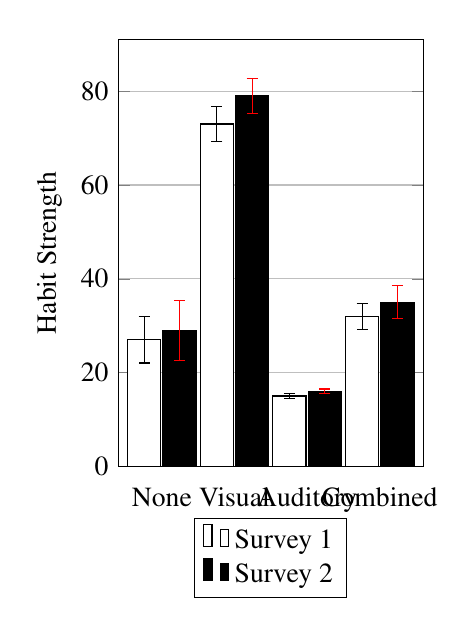
\begin{tikzpicture}
   \begin{axis}[
      width  = 0.45*\textwidth,
      height = 7cm,
      major x tick style = transparent,
      ybar=2*\pgflinewidth,
      bar width=12pt,
      ymajorgrids = true,
      symbolic x coords={None,Visual,Auditory,Combined},
      xtick = data,
      scaled y ticks = false,
      enlarge x limits=0.20,
      ymin=0,
      legend cell align=left,
      legend style={at={(0.5,-0.12)},anchor=north},
%       x label style={at={(axis description cs:0.5,-0.1)},anchor=north},
%       y label style={at={(axis description cs:-0.1,.5)},rotate=90,anchor=south},
%       xlabel={$u$ unemployment},
      ylabel={Habit Strength},
   ]
      \addplot[style={fill=white},error bars/.cd, y dir=both, y explicit]
          coordinates {
          (None, 27) += (0,4.950) -= (0,4.950)
          (Visual, 73) += (0,3.701) -= (0,3.701)
          (Auditory, 15) += (0,0.5) -= (0,0.5)
          (Combined, 32) += (0,2.828) -= (0,2.828)
          };

      \addplot[style={fill=black},error bars/.cd, y dir=both, y explicit,error bar style=red]
           coordinates {
           (None, 29) += (0,6.364) -= (0,6.364)
           (Visual, 79) += (0,3.701) -= (0,3.701)
           (Auditory, 16) += (0,0.5) -= (0,0.5)
           (Combined, 35) += (0,3.536) -= (0,3.536)
           };

      \legend{Survey 1, Survey 2}

  \end{axis}
  \end{tikzpicture}
  \caption{Comparing Habit strength verses reward type - the SRHI 4-item subset for Visual and Visual with Auditory modalities.}~\label{fig:habit_4_item_survey1_v_survey2}
\end{figure}

\subsubsection{Limitations}
TODO: Facebook limitations. Briefly discuss vibration limitations.






\section{Discussion}
TODO: Compare these results to people not using the chatbot, e.g.. people signing up to the gym, new years resolution

\subsection{Questions}
\subsubsection{Did users like the bot?}
Yes: Well the number of snoozes over time decreased (chart), the number of total habits completed per day decreased for all reward types (including the control group)~\ref{fig:allhabits_v_rewards} and users streaks over time increased (chart). In addition, 36 people used it for 3-weeks. Also 31 participants actually completed a habit or marked one as not yet and 31 participants interacted with the bot at least once.




\subsubsection{Were the rewards motivating?}
Not really: The graphs show that the number of snoozes for all modalities stays roughly the same, except for the control group which declines.


\subsubsection{Was chatbot successful at running a trial?}
TODO: Did have a lot of issues, but did get a lot of data.


\subsection{Limitations}
There are x key limitations to these findings. Firstly, the small number of participants and the small sample of rewards used in the study make it unclear how these findings would generalise to other types of rewards with the same modality.

TODO: Say we are aware of other types of rewards, but we chose positive reinforcement (intrinsic? ex? reward)




\section{Conclusions and Future Work}

% CHI Contributions:
%   - Build bot because of implementation reasons and social support from social network
%     - If a bot pretends to be a person, you more likely to respond as a person, as social scaffolding
%   - Design recommendations, this is what we have learnt, if you are going to design chatbots, these are my recommendations

This paper presents two contributions: i) design guidelines for designing habit formation chatbots that focus on rewards from different modalities, ii) analysis about how rewards delivered-by-a-bot from different modalities effect habit strength.

We encourage the use of these results to compare with different types of rewards for behaviour change technology. We hope this opens up new research avenues for investigating the use of chatbots as vehicles for promoting behaviour change.


\section{Acknowledgements}
We thank all the participants involved, the internal reviewers and staff who provided helpful feedback throughout the trial.


\subsection{Other Results}
(NOTE: I am not sure if I should include any of these)

\subsubsection{What was users habit context?}
31 participants (86\%) chose one of the contexts that were listed as examples, some with a slight change in before and after wording, e.g. before getting home from work, rather than after getting home from work. The remaining 5 people chose the following context: 'Having a snack', 'Sitting in bed', 'Early morning', 'during breakfast' and 'Before sleeping'.

Suggested habit contexts (by the bot):(todo insert table: morning, afternoon, evening habit context)

Morning:
  - waking up
  - eating breakfast
  - arriving at work

  Afternoon:
  - eating lunch
  - leaving work

  Evening:
  - leaving work
  - eating dinner
  - getting ready for bed

  Morning: 100: 7 (early) + 66 (mid) + 27 (late)
  Afternoon: 54: 7 + 4 + 43
  Evening: 32: 6 + 15 + 11


\subsubsection{How many people previously used habit tracking systems before?}
7 people (19\%) used them before and 100\% of those people said they worked. They tracked habits such as 'Diet' (3 people), 'Exercise' (3 people), 'Deadlines' (2 people), 'Audiobook reading' (1), 'Weight' (1). These people all chose new habits that they hadn't listed that they had tracked before.

\subsubsection{What is the highest streaked habit?}
Meditation had the most cumulative streak (17) followed by stretching (7 people).

\subsubsection{What is the correlation between reward and streaks?}
High streaks (streak over 10) had habits: meditation (total 135 streaks) and stretch (126 streaks). Rewards wise, VISUAL AND SOUND had the most streaks (126 combined), control group 75, then VISUAL (60)


\subsubsection{What was the habit that lasted the longest?}
Stretch had the highest streak (18), meditation (15). However, overall, for all habits completed, meditation was the most streaked (269 combined), stretching (231 combined), then press ups (39) then plank (24)

\subsubsection{Failed snoozes}
Visual and sound had the most number of failed snoozes (10, split over 6 people, 1 person had 5 failed snoozes). Then it was sound by 4.

\subsubsection{Users issues they had}

\begin{itemize}
  \item x7 People tried to message to bot instead of using the quick replies
  \item x1 People tried to send multiple messages for free input, rather than all in a single message
  \item x1 Endless loop with different type
  \item x1 People tried to respond to the multiple messages with a thumb.
\end{itemize}


\subsubsection{Users feedback they gave in an unconventional way}
Feedback users gave when they just randomly messaged the bot.

\begin{itemize}
  \item Asked: What kind of thing are you looking to find out?
  \item Asked: 'Don't that will be annoying' when asked about being messaged every day
  \item Asked: 'Never' when asked about being messaged every day
  \item Asked: 'This is not working for me', got no response.
  \item Asked: 'Lame same band' when got same reward twice
  \item Asked: 'stop', then blocked the bot
  \item 1 user press a thumb to say they completed a habit
\end{itemize}

For example, during the pilot trials when asking for an existing routine, users were confused, so examples of habit contexts were provided. The results found, 92?\% of participants chose one of these examples.
31 people chose one of the contexts that were listed as examples, some with a slight change in before and after wording, e.g. before getting home from work, rather than after getting home from work. The remaining 5 people chose the following context: 'Having a snack', 'Sitting in bed', 'Early morning', 'during breakfast' and 'Before sleeping'.



% % Either:
% %  1. Put \balance{} in the first column of the last page
% %  2. Don't use \balance{}
% %  3. hard-code a column break into the bbl file (before submission)
% % see more http://stackoverflow.com/questions/2149854/how-to-manually-equalize-columns-in-an-ieee-paper-if-using-bibtex
% \balance{}


\bibliographystyle{scaffold/SIGCHI-Reference-Format}
\bibliography{sample}

\end{document}
